% --------------------------------------------------------------------------- %
% Poster for the ECCS 2011 Conference about Elementary Dynamic Networks.      %
% --------------------------------------------------------------------------- %
% Created with Brian Amberg's LaTeX Poster Template. Please refer for the     %
% attached README.md file for the details how to compile with `pdflatex`.     %
% --------------------------------------------------------------------------- %
% $LastChangedDate:: 2011-09-11 10:57:12 +0200 (V, 11 szept. 2011)          $ %
% $LastChangedRevision:: 128                                                $ %
% $LastChangedBy:: rlegendi                                                 $ %
% $Id:: poster.tex 128 2011-09-11 08:57:12Z rlegendi                        $ %
% --------------------------------------------------------------------------- %
\documentclass[a0paper,portrait]{baposter}

\usepackage{relsize}		% For \smaller
\usepackage{url}			% For \url
\usepackage{epstopdf}	% Included EPS files automatically converted to PDF to include with pdflatex
\usepackage{booktabs}
\usepackage{color}
\usepackage{graphicx}
\usepackage{subfigure}
\usepackage{comment}
\usepackage[fleqn]{amsmath}
\usepackage{multirow}
\usepackage{comment}
%%% Global Settings %%%%%%%%%%%%%%%%%%%%%%%%%%%%%%%%%%%%%%%%%%%%%%%%%%%%%%%%%%%

\graphicspath{{pix/}}	% Root directory of the pictures 
\tracingstats=2			% Enabled LaTeX logging with conditionals

%%% Color Definitions %%%%%%%%%%%%%%%%%%%%%%%%%%%%%%%%%%%%%%%%%%%%%%%%%%%%%%%%%

\definecolor{bordercol}{RGB}{40,40,40}
\definecolor{headercol1}{RGB}{186,215,230}
\definecolor{headercol2}{RGB}{80,80,80}
\definecolor{headerfontcol}{RGB}{0,0,0}
\definecolor{boxcolor}{RGB}{186,215,230}

%%%%%%%%%%%%%%%%%%%%%%%%%%%%%%%%%%%%%%%%%%%%%%%%%%%%%%%%%%%%%%%%%%%%%%%%%%%%%%%%
%%% Utility functions %%%%%%%%%%%%%%%%%%%%%%%%%%%%%%%%%%%%%%%%%%%%%%%%%%%%%%%%%%

%%% Save space in lists. Use this after the opening of the list %%%%%%%%%%%%%%%%
\newcommand{\compresslist}{
	\setlength{\itemsep}{1pt}
	\setlength{\parskip}{0pt}
	\setlength{\parsep}{0pt}
}

%%%%%%%%%%%%%%%%%%%%%%%%%%%%%%%%%%%%%%%%%%%%%%%%%%%%%%%%%%%%%%%%%%%%%%%%%%%%%%%
%%% Document Start %%%%%%%%%%%%%%%%%%%%%%%%%%%%%%%%%%%%%%%%%%%%%%%%%%%%%%%%%%%%
%%%%%%%%%%%%%%%%%%%%%%%%%%%%%%%%%%%%%%%%%%%%%%%%%%%%%%%%%%%%%%%%%%%%%%%%%%%%%%%

\begin{document}
\typeout{Poster rendering started}

%%% Setting Background Image %%%%%%%%%%%%%%%%%%%%%%%%%%%%%%%%%%%%%%%%%%%%%%%%%%
\background{
	\begin{tikzpicture}[remember picture,overlay]%
	\draw (current page.north west)+(-2em,2em) node[anchor=north west]
	{\includegraphics[height=1.1\textheight]{background}};
	\end{tikzpicture}
}

%%% General Poster Settings %%%%%%%%%%%%%%%%%%%%%%%%%%%%%%%%%%%%%%%%%%%%%%%%%%%
%%%%%% Eye Catcher, Title, Authors and University Images %%%%%%%%%%%%%%%%%%%%%%
\begin{poster}{
	grid=false,
	% Option is left on true though the eyecatcher is not used. The reason is
	% that we have a bit nicer looking title and author formatting in the headercol
	% this way
	%eyecatcher=false, 
	borderColor=bordercol,
	headerColorOne=headercol1,
	headerColorTwo=headercol2,
	headerFontColor=headerfontcol,
	% Only simple background color used, no shading, so boxColorTwo isn't necessary
	boxColorOne=boxcolor,
	headershape=roundedright,
	headerfont=\Large\sf\bf,
	textborder=rectangle,
	background=user,
	headerborder=open,
  boxshade=plain
}
%%% Eye Cacther %%%%%%%%%%%%%%%%%%%%%%%%%%%%%%%%%%%%%%%%%%%%%%%%%%%%%%%%%%%%%%%
{
	Eye Catcher, empty if option eyecatcher=false - unused
}
%%% Title %%%%%%%%%%%%%%%%%%%%%%%%%%%%%%%%%%%%%%%%%%%%%%%%%%%%%%%%%%%%%%%%%%%%%
{\sf\bf
	Fish recognition using deep convolutional neural network and data augmentation
}
%%% Authors %%%%%%%%%%%%%%%%%%%%%%%%%%%%%%%%%%%%%%%%%%%%%%%%%%%%%%%%%%%%%%%%%%%
{
	\vspace{1em} Ziqiang Zheng, Chao Wang, Zhibin Yu, Haiyong Zheng, Weiwei Wang\\
	{\smaller zhengziqiang1@gmail.com, wangchaoplus@gmail.com, yuzhibin@ouc.edu.cn, zhenghaiyong@ouc.edu.cn, 17854206960@163.com}
}
%%% Logo %%%%%%%%%%%%%%%%%%%%%%%%%%%%%%%%%%%%%%%%%%%%%%%%%%%%%%%%%%%%%%%%%%%%%%
{
% The logos are compressed a bit into a simple box to make them smaller on the result
% (Wasn't able to find any bigger of them.)

\setlength\fboxsep{0pt}
\setlength\fboxrule{0.5pt}
	\fbox{
		\begin{minipage}{10em}
%			\includegraphics[width=10em,height=4em]{colbud_logo}
%			\includegraphics[width=4em,height=4em]{elte_logo} \\
%			\includegraphics[width=10em,height=4em]{dynanets_logo}
%			\includegraphics[width=4em,height=4em]{aitia_logo}
			
\includegraphics[width=10em,height=10em]{logo_resize}
		\end{minipage}
	}
}
%
\includegraphics[width=\linewidth]{logo_resize}


\headerbox{Problem}{name=problem,column=0,row=0}{
\quad Nowadays, as a sub topic of computer vision and fishery industry, fish recognition is still a challenging work not only because of various kinds of fish, but also because of the complex background of images.

%\includegraphics[width=\linewidth]{time_windows}
}

\headerbox{Introduction}{name=definitions,column=0,below=problem}{
\quad In this paper, we will introduce two methods to improve the classification accuracy. We have done some data preprocessing before training our model. First we make a mask in the fish region and make the fish region black, which we regard as the NoF fish images. Then we use some methods to achieve data augmentation. At last we use the convolutional neural network (CNN) as the classifier. The first method is based on data augmentation. The second improvement is based on some image preprocessing methods. We have made a mask of the area where the fish are located, and we have used both the processed images and the raw images to train our model.
\begin{center}
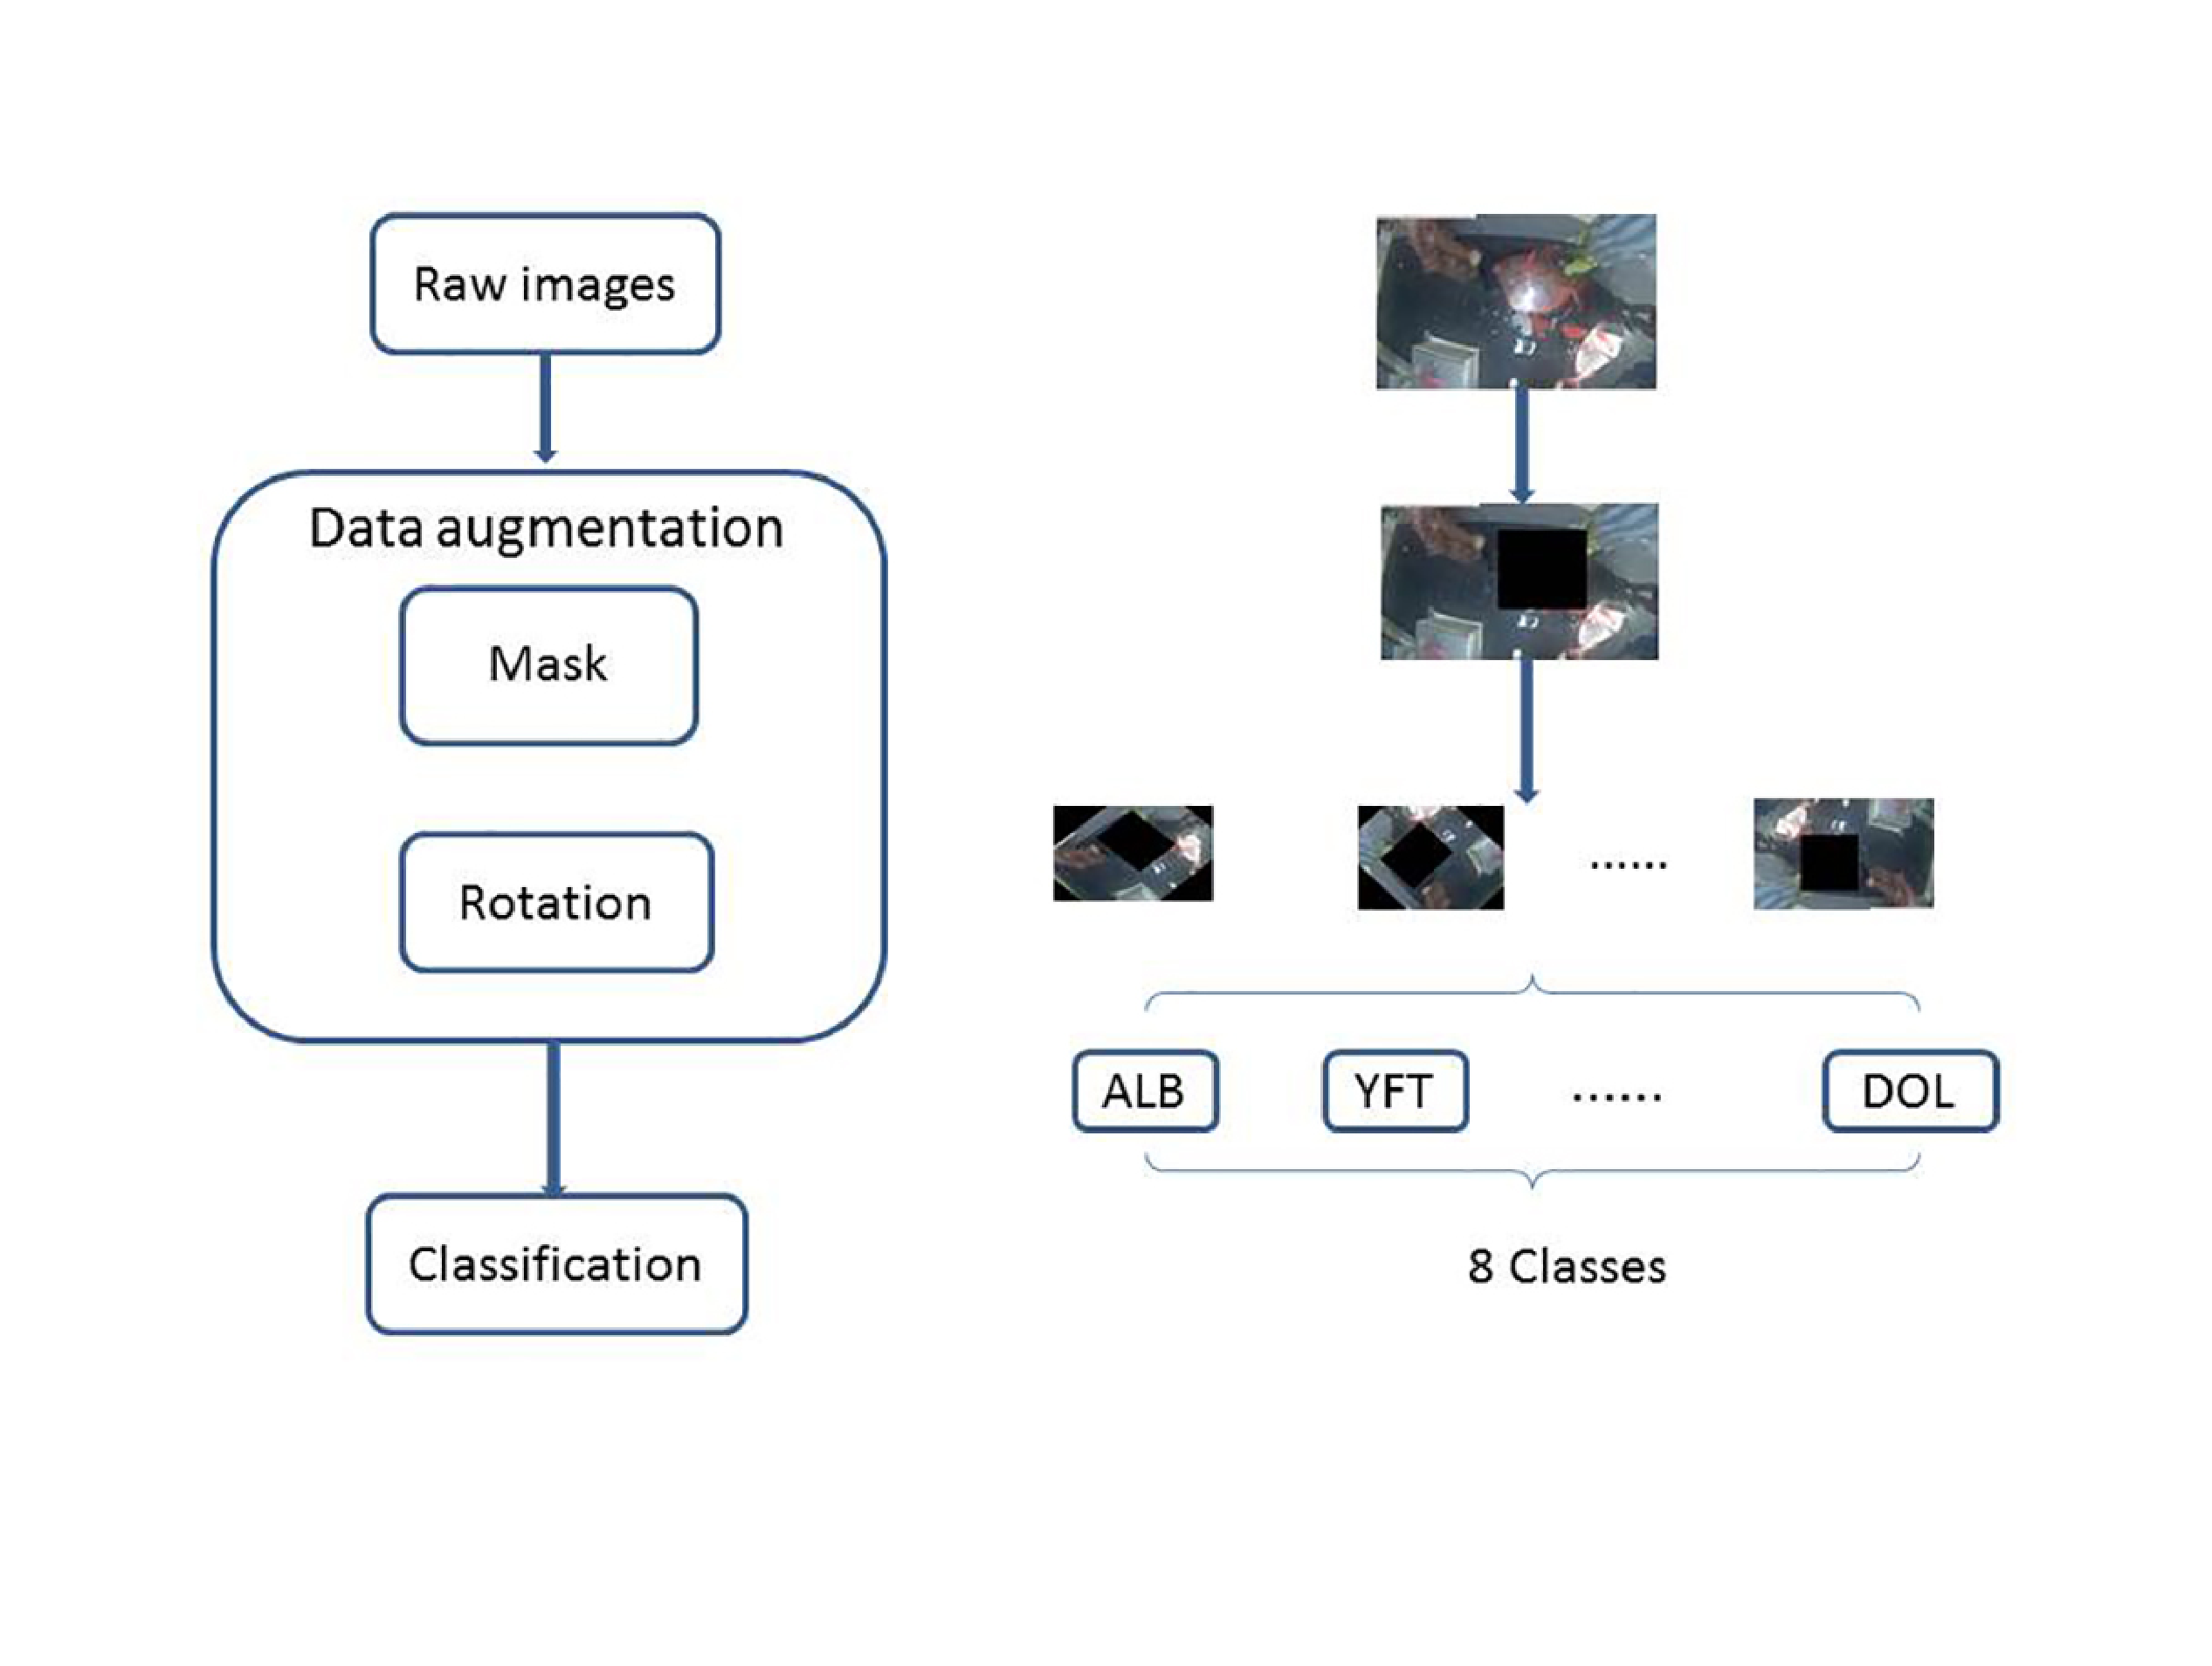
\includegraphics[width=0.9\linewidth]{demo}
\end{center}
}



\headerbox{Experiments}{name=models,column=0,below=definitions}{
\quad The table shows the test loss in the Kaggle competition. We mainly have used two different architectures of networks. The first two columns indicate the benchmark. By comparing the test loss when using the two methods with the benchmark, we can see that the rotating method and mask method both have decreased the test loss.\\
\\
\begin{tabular}{l l l l}
\toprule
\textbf{Method} & \textbf{Model} & \textbf{Test loss} \\
\midrule
	None	& Caffenet	& 1.92 \\
       None	& GoogleNet	& 2.56 \\
       Rotating & Caffenet     & 1.77  \\
       Rotating & GoogleNet   & 1.93    \\
	Mask	& Caffenet	& 1.87   \\
	Mask	& GoogleNet	& 2.25    \\
	Rotating + Mask &Caffenet & 1.71   \\
	Rotating + Mask &GoogleNet & 1.85  \\
\bottomrule
\end{tabular}



}

\headerbox{References}{name=references,column=0,below=models}{
\smaller													% Make the whole text smaller
\vspace{-0.4em} 										% Save some space at the beginning
\bibliographystyle{plain}							% Use plain style
\renewcommand{\section}[2]{\vskip 0.05em}		% Omit "References" title
\begin{thebibliography}{1}							% Simple bibliography with widest label of 1
\itemsep=-0.01em										% Save space between the separation
\setlength{\baselineskip}{0.4em}					% Save space with longer lines
\bibitem{prevWork1} Sharif Razavian, Ali and Azizpour, Hossein and Sullivan et al.: \emph{CNN features off-the-shelf: an astounding baseline for recognition}, Proceedings of the IEEE Conference on Computer Vision and Pattern Recognition Workshops (2014) 
\bibitem{prevWork2} Krizhevsky, Alex and Sutskever, Ilya et al.: \emph{Imagenet classification with deep convolutional neural networks}, Advances in neural information processing systems (2012)
\bibitem{gulya-kampis1} Jia, Yangqing and Shelhamer, Evan and Donahue et al.: \emph{Caffe: Convolutional Architecture for Fast Feature Embedding}, arXiv preprint arXiv:1408.5093 (2014)
\end{thebibliography}
}


\headerbox{Main Methods}{name=density,span=2,column=1,row=0}{
%Network characteristics are extremely sensitive to minor changes in aggregation length. In our previous work \cite{prevWork1} \cite{prevWork2}, we studied the cumulative properties of Elementary Dynamic Network models over the complete time period (i.e., until they reach the stable point of a full network). Here we focus on the more realistc domain of sparse (cumulative) networks. We find that even when snapshot networks are stationary, \textbf{important network characteristics}  (average path lenght, clustering, betwenness centrality) \textbf{are extremely sensitive to aggregation} (window length). 

\quad The architecture of our model used in the experiment is the convolutional neural network, which has achieved remarkable performance in image classification and object detection recently\cite{prevWork1}\cite{prevWork2}. There still exists the problem that our model can't distinguish between foreground and background. We make a mask of the area where the fish are located, because the mask can force our model to concentrate on the fish area by comparing the raw images and the processed images. So it can help our convolutional neural network detect the fish region. We have trained our model using both the two images at the same time, which can improve the robustness of the fish recognition.In consideration of the imbalance of the dataset, we got some new images by rotating the selected images. Through this method, we can increase the number of some species of fish images, which can help avoid that our model is over-fitted with some categories of fish images, and rotating the fish images can improve the robustness of detection and achieve sophisticated detection.
\\
\\
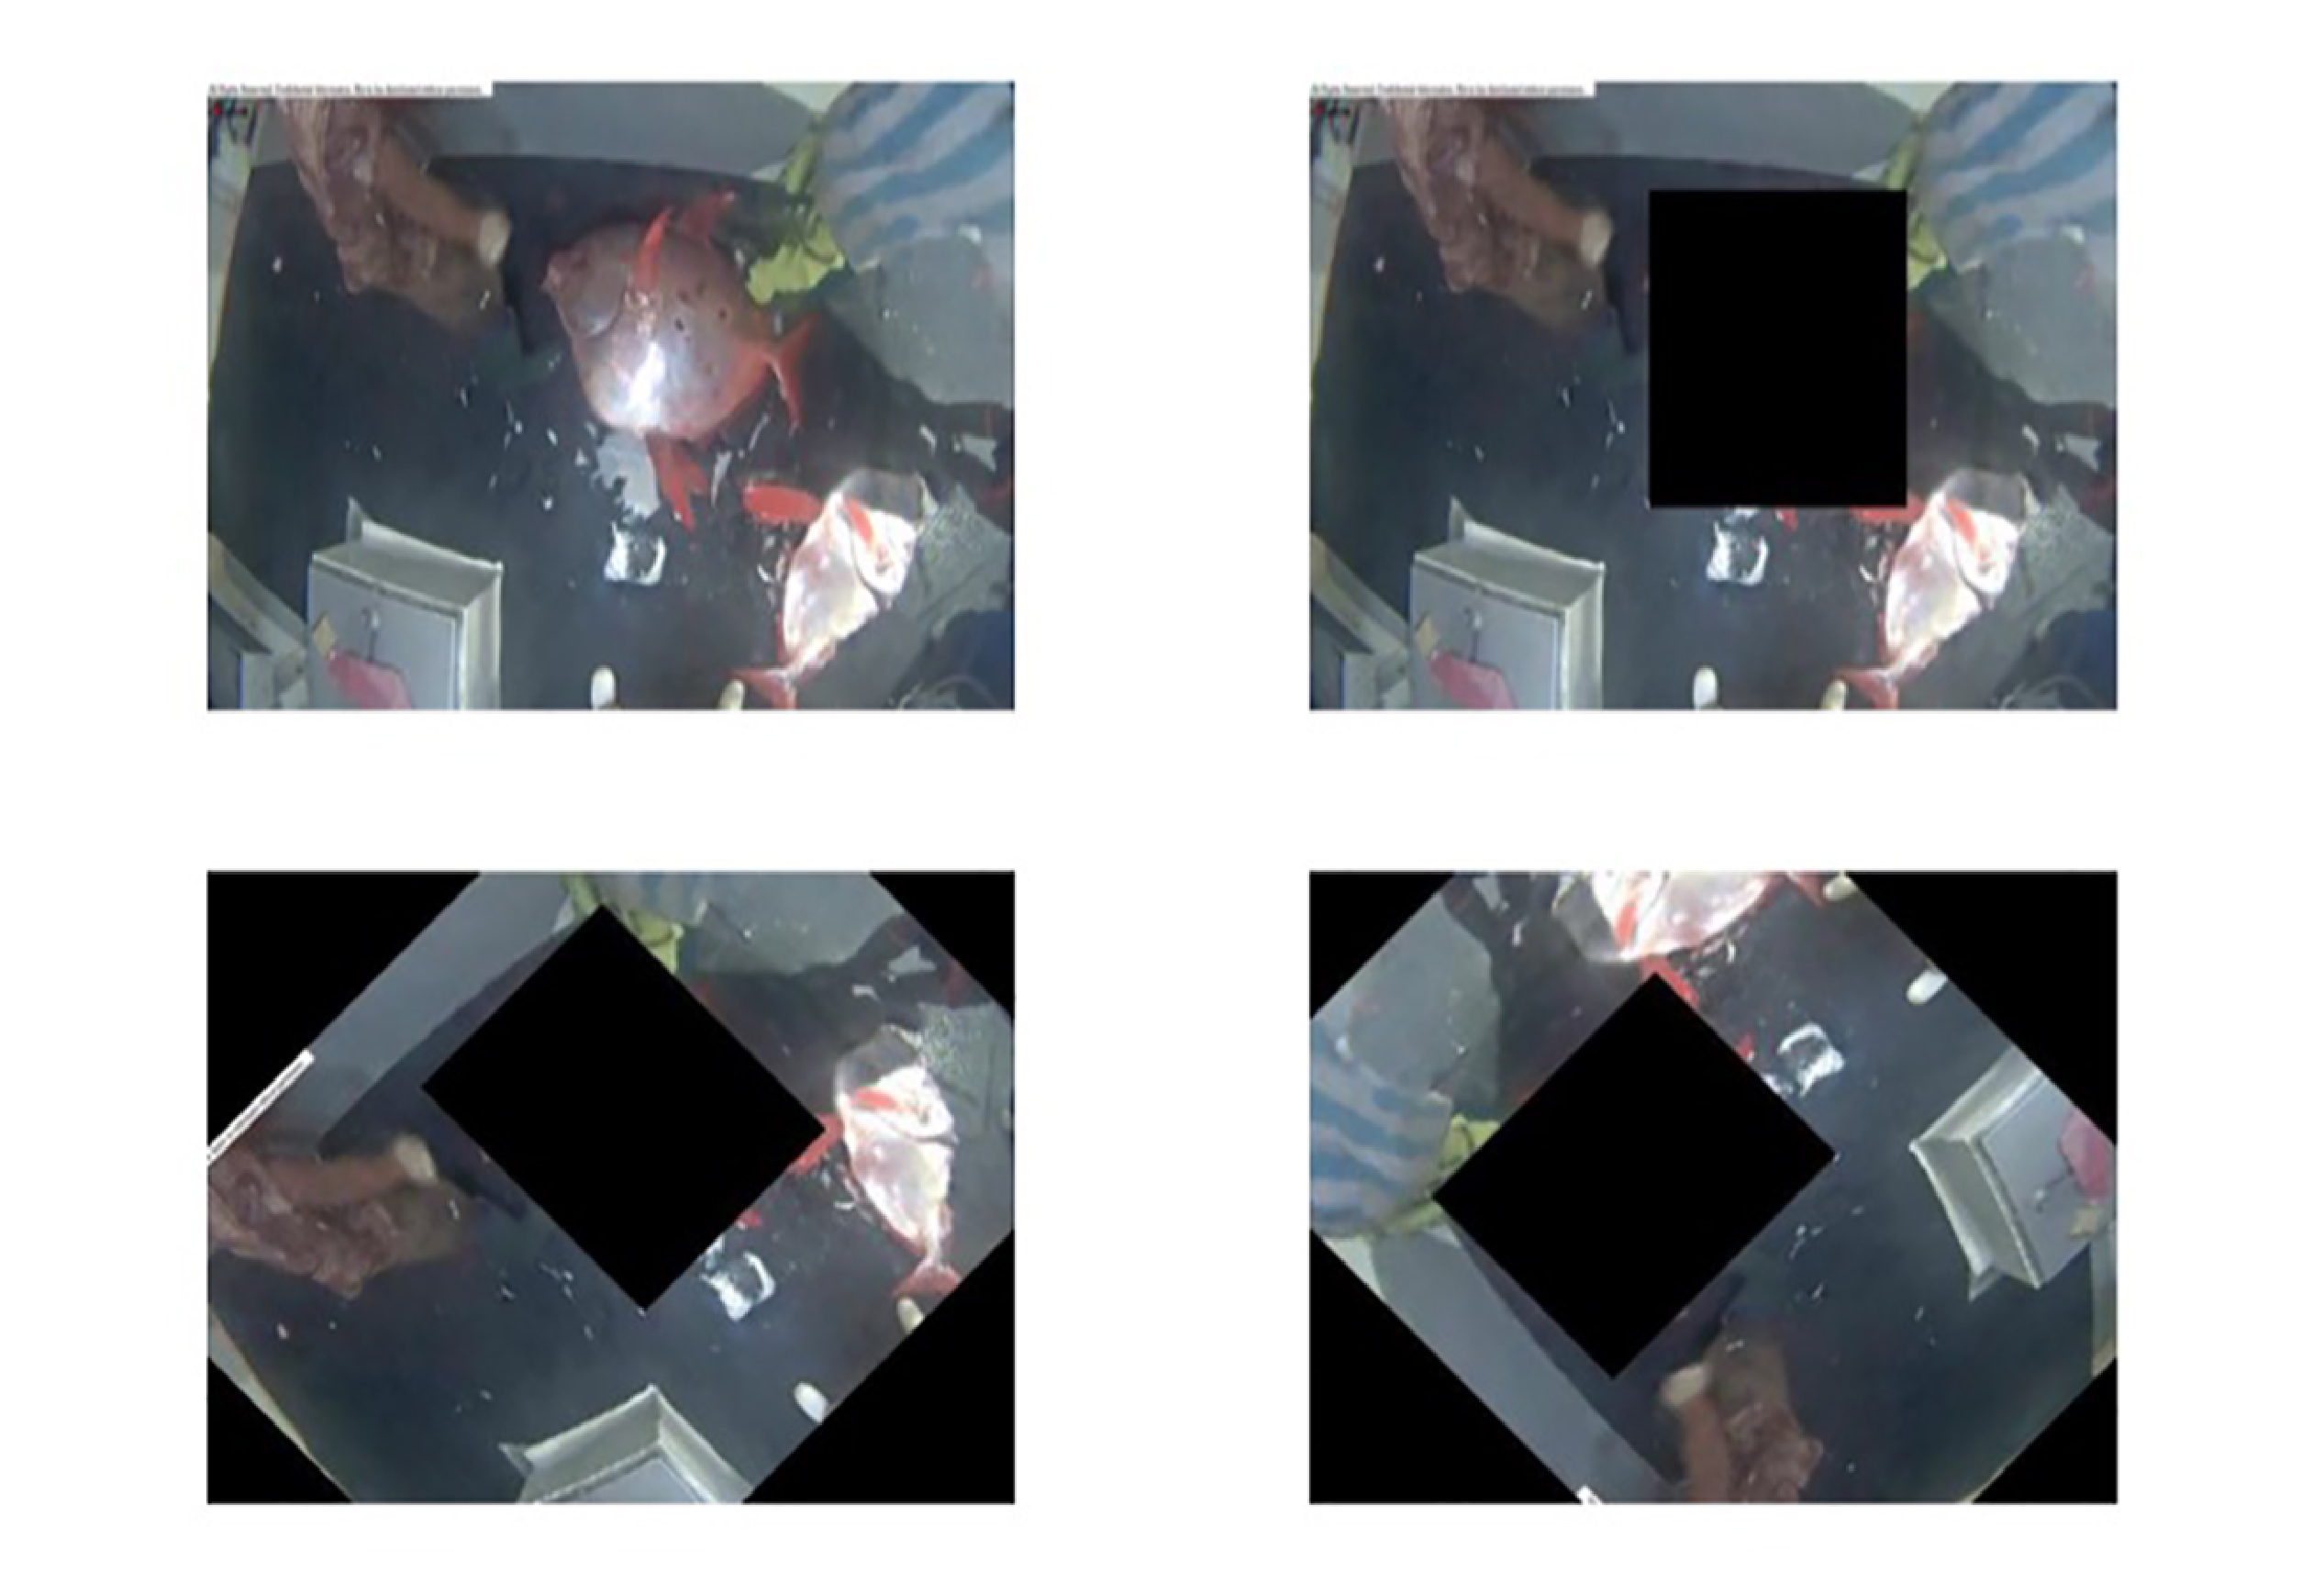
\includegraphics[width=\linewidth]{11}
}

\headerbox{Result Verification}
{name=degreeDistribution,span=2,column=1,below=density,above=bottom}{
%Degree distributions are exceptionally sensitive to the length of the aggregation window. \textbf{The same dynamic network may produce a normal, lognormal or even power law distribution for different aggregation lenghts.} The digree distribution of the snapshot and cumulative network is inherently different. The following surfaces show the CPA model until it approaches the complete network.
\quad In order to prove that the fish region has really made contribution in the fish recognition, we modified Caffe\cite{gulya-kampis1} to get the pooling images. And the figure shows the comparison between the raw images and the pooling images. In consideration of the big number of the pooling images, we have picked up 36 pooling images from 64 pooling images and resized each of all to merge them into one image. From the two sets of images, we can see that the fish region is brighter than other regions in most of the pooling images.

\vspace{-0.2em}
\begin{center}
%	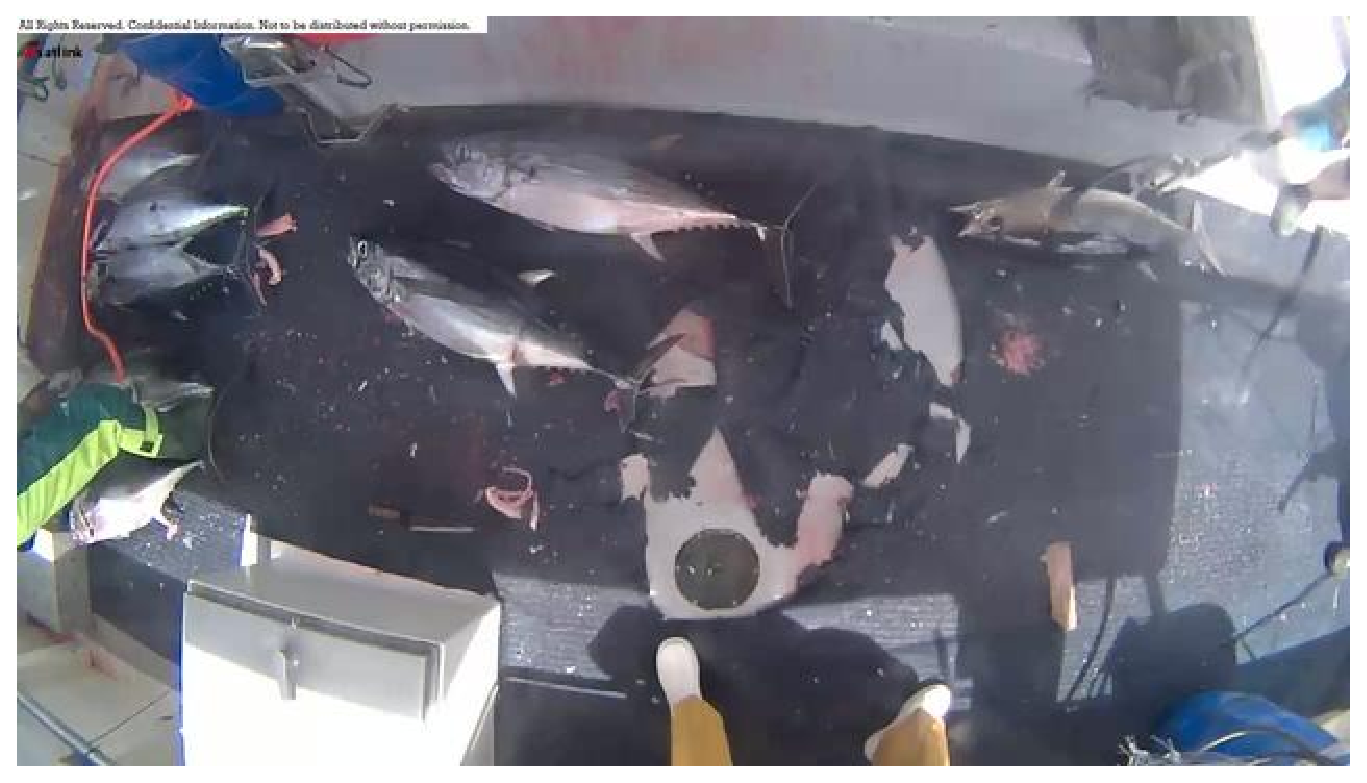
\includegraphics[angle=-90,width=0.49\linewidth]{resize}
%	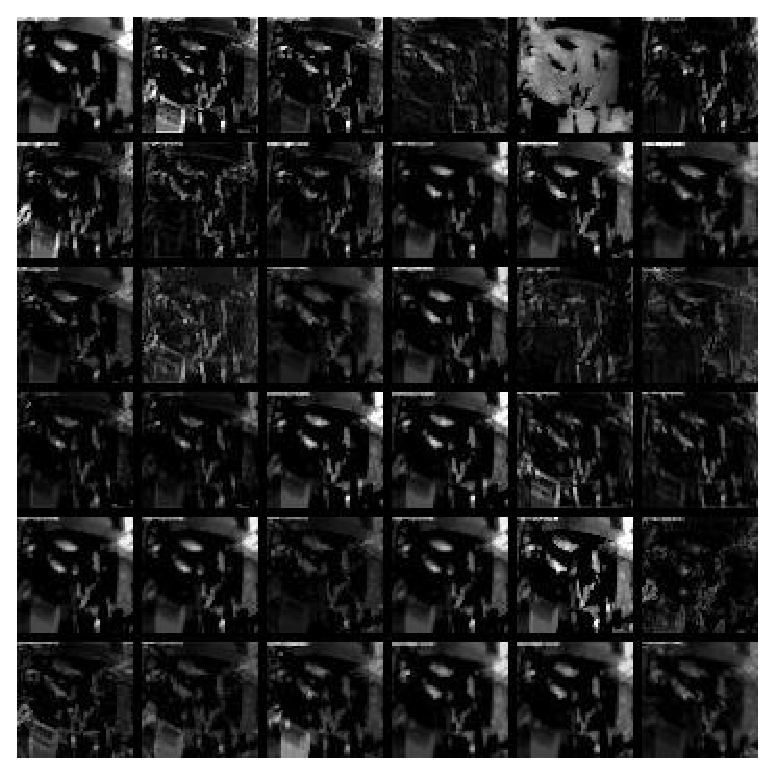
\includegraphics[angle=-90,width=0.49\linewidth]{merge_2}
	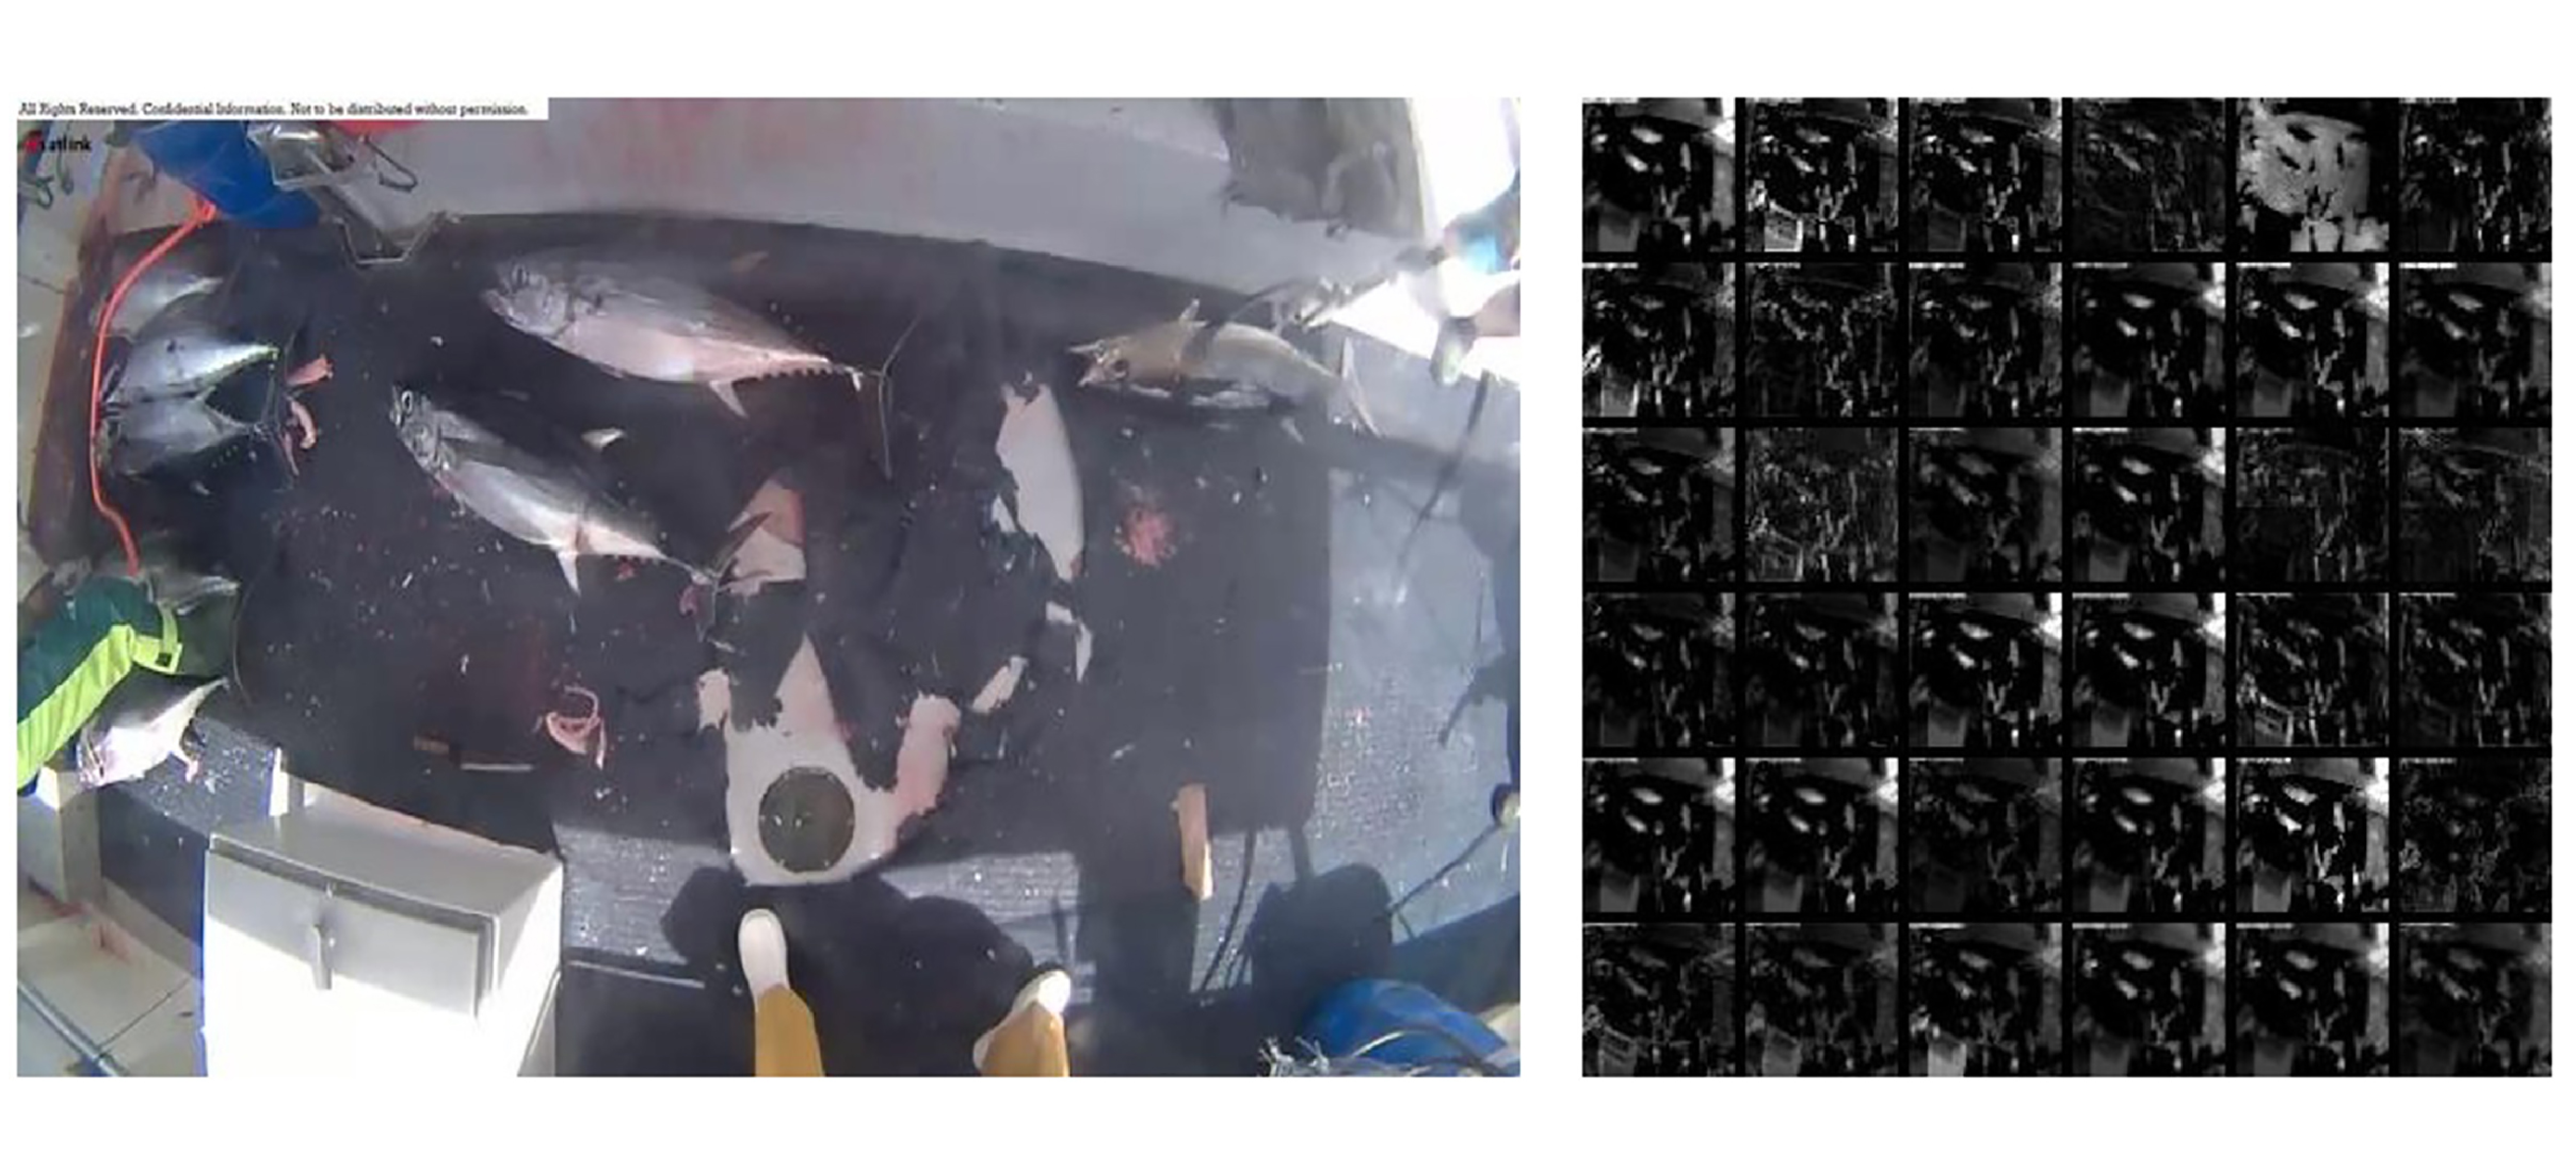
\includegraphics[width=\linewidth]{merge}
\end{center}
\vspace{-0.2em}
\quad From the two sets of images, we can see that the fish region is brighter than other regions in most of the pooling images, and this proves that fish make more contribution than the background for the classification. Our research can benefit the development of the marine resources, as well as commercial applications such as fisheries and aquaculture.
%\vspace{-0.2em}
%\begin{center}
%	\includegraphics[angle=-90,width=0.49\linewidth]{ER1_cumulativeDegrees}
%	\includegraphics[angle=-90,width=0.49\linewidth]{CPA_cumulativeDegrees}
%\end{center}
}

\end{poster}
\end{document}
